 % !TEX encoding = UTF-8 Unicode

\documentclass[a4paper]{article}

\usepackage{color}
\usepackage{url}
\usepackage[T2A]{fontenc} % enable Cyrillic fonts
\usepackage[utf8]{inputenc} % make weird characters work
\usepackage{graphicx}

\usepackage[english,serbian]{babel}
%\usepackage[english,serbianc]{babel} %ukljuciti babel sa ovim opcijama, umesto gornjim, ukoliko se koristi cirilica

\usepackage[unicode]{hyperref}
\hypersetup{colorlinks,citecolor=green,filecolor=green,linkcolor=blue,urlcolor=blue}

%\newtheorem{primer}{Пример}[section] %ćirilični primer
\newtheorem{primer}{Primer}[section]

\begin{document}

\title{Sajber rat\\ \small{Seminarski rad u okviru kursa\\Računarstvo i društvo\\ Matematički fakultet}}

\author{Luka Vukotić\\ mi19120@alas.matf.bg.ac.rs}
\date{02.~septembar 2022.}
\maketitle

\abstract{

Dati su odgovori na pitanja kako
definisati sajber rat, kada, kako i zašto se on javlja. Pokazani su neki
(navodni) primeri sajber ratovanja. Predstavljene su neke metode koje se
koriste za napade u sajber prostoru, kao i uzorak heurističkog dijagrama
za klasifikaciju tipova sajber napada. Dati su slikoviti primeri same anatomije i konstrukcije samih sajber napada, kao i razlozi za sve veći broj ljudi koji se bave sajber kriminalom a koji su verovatno uključeni u neki vid sajber rata. Takođe, u ovom radu su prikazane i najpopularnije vrste sajber napada kao i neki od načina njihove prevencije. Pored priče o sajber ratu i napadima na globalnom nivou poslednji segment ovog rad je posvećen sajber napadima u Srbiji kao i spremnosti naše države da odgovori na ovu sve učestaliju pojavu.


\tableofcontents

\newpage

\section{Uvod}
\label{sec:uvod}
Sajber rat je potajan i nevidljiv za većinu. Naime on se odvija u sajber prostoru koga čine sve računarske mreže na svetu. \textbf{Sajber-prostor} se često definiše i kao peto ratno područje posle kopna, mora, vazduha i svemira za koje si već znamo.
Termin sajber rata je korišćen u mnogim različitim kontekstima, ali u većini slučajeva sa sobom ne povlači neki vid nasija na koji smo kroz istoriju navikli kada pomenemo samu reč rat. Sajber rat može uključivati kinetičke i nekinetičke aktivnosti:
\begin{itemize}
\item Pod pojmom kinetičke aktivnosti mislimo na aktivnosti koje se povezuju sa nekim vidom kretanja (npr. pokretanje vojnih snaga, bacanje bombi i korišćenje vojnog naoružanja u nekom području).
\item Nekinetičke aktivnosti su uglavnom usmerene ka bilo kom pristupu suparničkim sajber sistemima, kao što su prisluškivanje, preuzimanje obaveštajnih podataka itd...;
\end{itemize} 

\section{Šta je sajber rat?}
Što se tiče neke univerzalne definicije ona još uvek ne postoji.
Naime, postoji značajna debata među ekspertima u ovoj oblasti o definiciji pojma sajber rata/ratovanja kao i da li tako nešto uopšte postoji. Postoji tu dosta problema koji se javljaju prilikom pronalaženja univerzalne definicije.
Prvi problem prilikom definisanja ovog pojma je to što sajber ratovanje ne ispunjava tipičnu definiciju rata, ali ipak mnoge države imaju aktivne sajber operacije za napad i odbranu. Pored već pomenutih problema, eksponencijalni rast inetrneta i internet tehnologija dovodi do toga da sajber napadi budu sve rasprostranjeniji, i u ovakvom okruženju uticaj zakona o sajber ratovanju može biti veoma ograničen.
Ipak iako ne postoji prihvaćena univerzalna definicija postoji više različitih definicija koje mogu biti kandidati:

\begin{itemize}
\item  Talinski priručnik definiše sajber rat kao sajber napad, u
odbranbenoj ili napadnoj sajber operaciji, koji rezultuje u
nasilju, smrti i/ili destrukciji. Nedostatak ove definicije -
isključuje npr. sajber operacije dizajnirane da destabilizuju
finansijski sistem nacionalne države
\item DCAF odnosno ženevski centar za demokratsku kontrolu oružanih snaga je usvojio sledeću definiciju: sajber rat je ratno ponašanje koje se sprovodi u virtuelnom svetu koristeći informacije, komunikacionu tehnologiju i mreže, sa namerom da poremeti ili uništi neprijateljske informacione i komunikacione sisteme;


\end{itemize} 




\section{Učestalost sajber napada}	
\label{sec:termini_i_citiranje}


Što se tiče učestalosti sajber napada praktično je nemoguće identifikovati/detektovati svaki sajber napad koji se dogodi.
Neki napadi se mogu neopaženo odvijati godinama (veoma napredan sistem) , drugi su kratkotrajni ali za sobom ne ostavljaju tragove pomoću kojih bi mogli biti otkriveni.
Takođe problem pravi i razvoj same tehnologije jer se sa razvojem povećava broj napada kao i njihova raznovrsnost, ali jedna od dobrih stvari je ta što se poboljšavaju i odbrambeni mehanizmi kao i sistemi za detekciju napada.  
Deutsche Telekom AG (DTAG), nemačka kompanija za telekomunikacije, uspostavila je mrežu od 97 senzora koji
služe kao sistem ranog upozorenja koji će u realnom vremenu pružiti  sliku o tekućem sajber napadima.
Iako je većina senzora smeštena u Nemačkoj, DTAG takođe locira honeypots\footnote{Honeypot je računarski sigurnosni mehanizam postavljen za otkrivanje, uklanjanje ili, na neki način, suzbijanje pokušaja neovlasćene upotrebe informacionih sistema.
}
i senzore u drugim neevropskim zemljama.
\newline
Top petnaest zemalja koje su DTAG senzori zabeležili kao izvor sajber napada istaknuti su na slici 1.
Otprilike 20\% navedenih sajber napada bilo je poreklom iz Ruske Federacije.
Prve četiri navedene države, uključujući SAD, Nemačku i Tajvan, činile su 62\% zastupljenih sajber napada.
Ovi slučajevi pružaju sliku napada usmerenih na određeno geografsko područje, u ovom slučaju Evropu.

 


\begin{verbatim}
\end{verbatim}

\begin{figure}[h!]
  \centering
  \begin{center}
  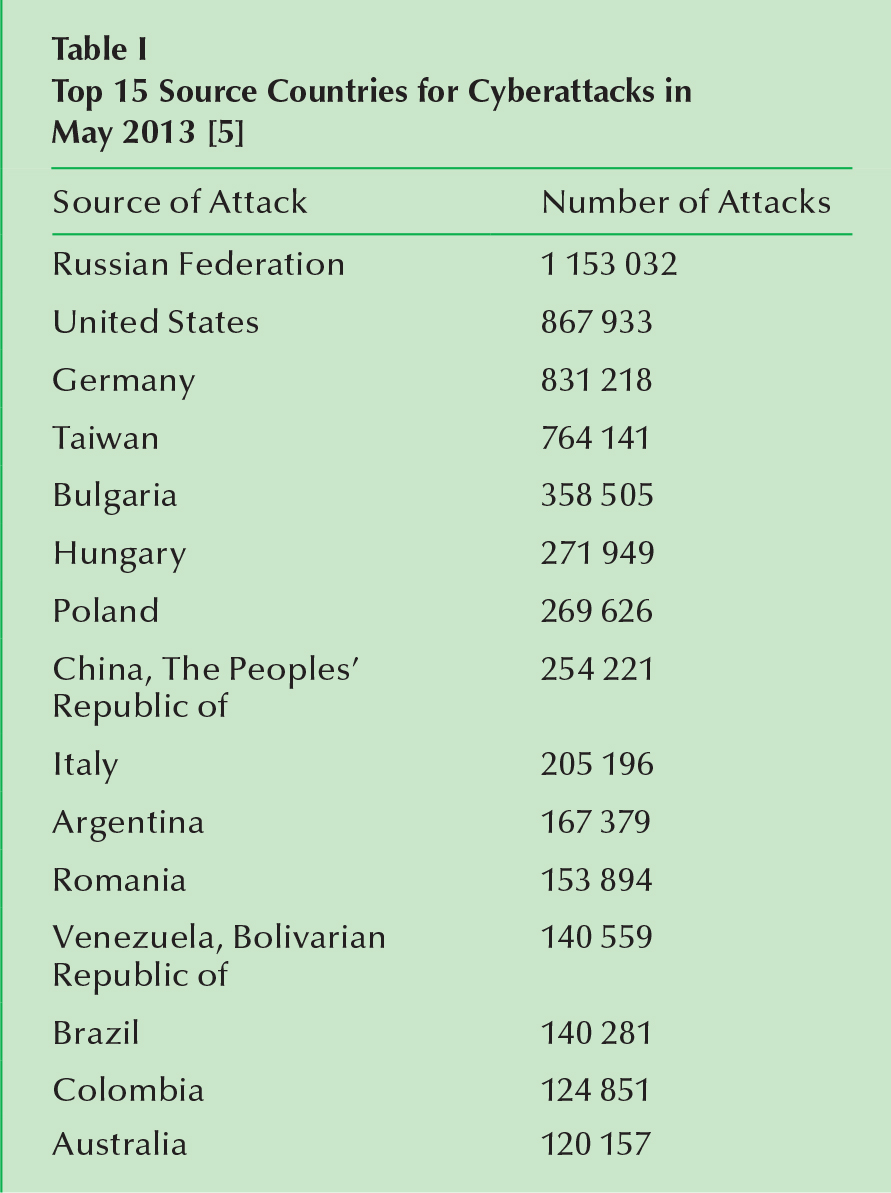
\includegraphics[width=55mm]{slika1.jpg}
  \end{center}
  \caption{Top 15 zemalja izvora za sajber napade u maju 2013. \cite{Overview of current cyber attacks}}
  \label{fig:vr1}
\end{figure}

\newpage

 



\section{Zašto se javlja sajber rat?}
\label{slike_i_tabele}


Za manje države ili terorističke oraganizacije upotreba DDoS (Distributed Denial of Service) napada je mnogo jeftinija (i takođe efikasnija) za pokretanje od konvencionalnih ratnih oružja i metoda napada protiv naprijatelja, koji uglavnom poseduje veći količinu resursa, vojne opreme, vojnih snaga, novca i generalno je veća vojna sila. Samom pojavom sajber rata pojavilo se i novo zanimanje pod nazivom sajber napadač. Sajber napadač za iznajmljivanje je profitabilan posao za one koji su ranije bili samo sajber kriminalci.
Kao što su primetili mnogi, sajber kriminalci mogu postati sajber ratnici za iznajmljivanje.
Ovaj lagani prelazak sa sajber kriminalca na sajber ratnika/napadača sugeriše to oslanjanje na strogo razgraničavanje između dve aktivnosti. Nije česta pojava i da školovani programeri poneseni novcem i materijalnom dobiti uplivaju u vode sajber kriminala što ćemo kasnije navesti u poglavlju o najpoznatijim zabeleženim sajber napadima. Pored same lakoće napada i količine uloženih resursa prilikom izvođenja napada, sajber napadi su takođe dosta efikasniji od konvencionalnih/kinetičkih napada. Takođe šteta koja se napravi prilikom sajber napada kao i prikupljene informacije mogu pomoći i u slučaju same kinetičke bitke. Primer za ovako nešto je onesposobljavanje raketne odbrane neke države koja je digitalno kontrolisana.
Sajber kriminal i sajber napadi mogu dugoročno dovesti do povećanja sajber napada.
Sami sajber napadi imaju sposobnost da poremete način života običnih ljudi (npr. haos koji bi se desio da se izvrši sajber napad na neki bankomat ili banku i račune u njoj). Takođe međusobna povezanost globalnih finansijskih institucija povećava rizik za sajber napad.
Ukoliko dođe do napada na neku od finansiskih filijala širom sveta moguće je preko nje pristupiti zaštićenim podacima iz drugih filijala koje su povezane sa hakovanom.








\section{Kako se javlja sajber rat?}
\label{sec:naslov1}


Većina ljudi je nekada čulo za neki od sajber napada koji su se dogodili u Srbiji ili svetu ali celokupna pozadina tog određenog događaja je u većini slučaja tajna ili skrivena. Naime, u većini slučajeva je pre jednog usepsnog napada više puta pokušan sajber napad sa istim ciljem ali različitim metodama. Kada navodimo sam pojam rata moraju da budu uključene dve strane koje se međusobno sukobljavaju. Veliki broj stručnjaka već godinama navodi kako se u sajber prostoru, tačnije putem sajber napada sprovodi treći svetski rat (uglavnom navode sukobe Ruske Federacije i Sjedinjenih Američkih Država), što je možda još uvek preuveličano ali samim razvojem tehnologije nema sumnje da će sajber napadi u budućnosti imati veliku ulogu u svim većim sukobima kako između država tako i između određenih korporacija koje jedna drugoj predstavljaju konkurenciju.

Prilikom sajber napada koriste se razni vektori, kako tehnosloski tako i organizacioni. Napadi traže ranjivost u bilo kom od delova koji čine sajber prostor. Istraživanjima je otkriveno da je veća verovatnoća da će određene vrste napada poteći iz određenih država i regiona. Na primer 75 procenata dobavljača internat usluga koji sadrže najviše phishing prevara potiču iz Sjedinjenih Američkih Država.


\begin{verbatim}
\end{verbatim}

\begin{figure}[h!]
  \centering
  \begin{center}
  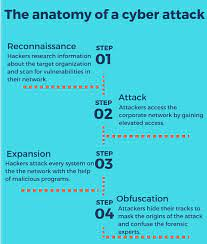
\includegraphics[width=55mm]{index.jpeg}
  \end{center}
  \caption{Slikovito prikazan proces sajber napada}
  \label{fig:vr1}
\end{figure}

\newpage

\section{Metode napada u sajber prostoru}
\label{sec:naslov2}

 \begin{figure}[h!]
  \centering
  \begin{center}
  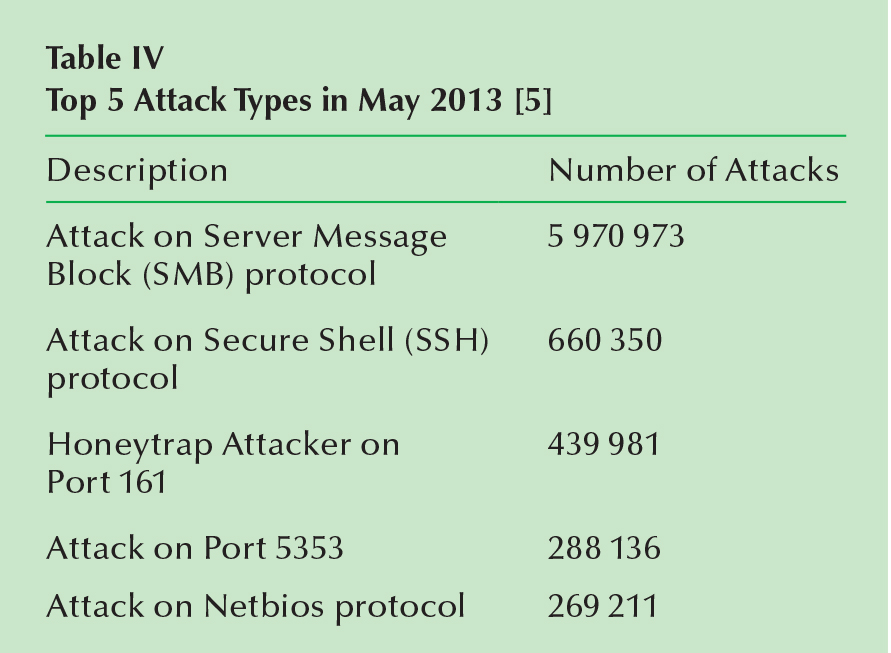
\includegraphics[width=55mm]{slika2.jpg}
  \end{center}
  \caption{Neke od zabeleženih metoda sajber napada}
  \label{fig:vr1}
\end{figure}


Kada pričamo o samim metodama napada u sajber prostoru njih ima neograničeno mnogo, jer se sa razvojem računarskih tehnologija povećava broj različitih načina samog napada. Veliki uticaj kada pričamo o metodama prilikom izvođenja sajber napada predstavljaju ciljevi samog sajber napada. Sajber napadi sa kojima se susreću obični ljudi u svakodnevnici mogu se nazvati nasumični napadi. Nasumični napadi se najčešće dešavaju u masovnim kampanjama gde nije targetirana jedna meta, već se malware plasira ka velikom uzorku meta svih dimenzija, a rezultat je po principu “ ko se upeca – upeca“. Ovakav tip napada primenjuju najčešće distributeri ransomware-a, botnet C&C-a itd gde je suština u masovnosti, ne u pojedinačnom cilju.
Targetirani napadi su dosta kompleksniji a samim tim zahtevaju i posvećenost napadača, gde je odvijanje celog napada unapred pripremano, kao i celokupna logistika njemu pridružena.

Na prikazanoj slici iznad se vidi 5 najpopularnijih vrsta napada otkrivenih u maju 2013te koje je otkrio sistem za identifikaciju napada koji je postavio DTAG. Kao što se sa slike može videti više od 50 procenata ovih napada je na Server Message Block protokolima.
Takođe SCADA sistemi su posebno osetljivi na sajber napade, a time i poprilično privlačni za sajber napadače. Naime SCADA, ili sistem nadzorne kontrole i prikupljanja podataka se koristi za kontrolu, praćenje i analizu industrijskih uređaja i procesa.
Sistem se sastoji od softverskih i hardverskih komponenti i omogućava daljinsko prikupljanje podataka kao i prikupljanje na licu mesta. Ovim sistemom se omogućava kompanijama da daljinski upravljaju industrijskim lokacijama kao što su na primer vetroparkovi itd...
Kako su SCADA sistemi sve više povezani sa drugim mrežama, uključujući i internet, samo povećavanje šanse za spoljašnju napad se prirodno dešava.



\section{Klasifikacija sajber napada}
\label{sec:naslovN}

\begin{figure}[h!]
  \centering
  \begin{center}
  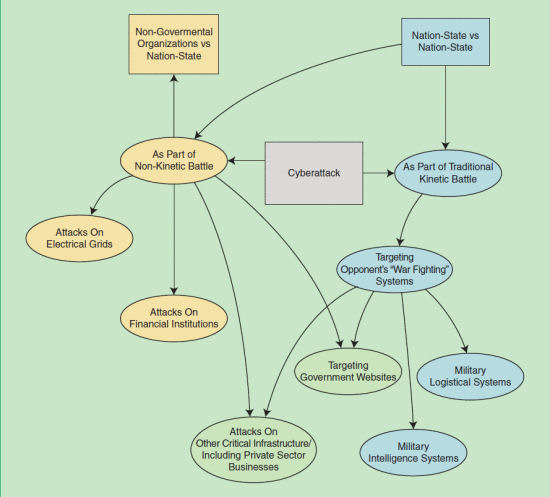
\includegraphics[width=55mm]{proces.jpg}
  \end{center}
  \caption{Proces odvijanja samog napada}
  \label{fig:vr1}
\end{figure}

Sajber napade možemo podeliti po nivoima pokretanja i nivoima na kojima može doći do sajber napada:
\begin{itemize}
    \item Vlada naspram vlade (u pogledu kinetičke bitke)
    \item Asimetrično ratovanje: nedržavni akter protiv sopstvenih agencija ili dobavljača, ili druge vlade (pod nedržavnim akterom se misli na razne terorističke grupe, političke grupe...)
    \item Vlada protiv kritične infrastrukture druge vlade
    \item  Krivično nadahnuti hakeri naspram pojedinačnih korisnika;
\end{itemize}



Pored ovakve podele možemo navesti i različite vrste napada po kojima ih možemo podeliti:
\begin{itemize}
    \item Phishing (pecanje) - napadi ove vrste su izuzetno česti i uključuju slanje velikih količina lažne elektronske pošte na ime nekog pouzdanog izvora (npr. vaša banka). Elektronske poruke često izgledaju kao legitimne, ali povezuju primaoca sa zlonamernom datotekom ili skriptom dizajniranom da omogući napadačima pristup vašem uređaju.
    \item MitM ili Man in the Middle - ova vrsta napada se javlja kada napadač presreće dvostranu transkaciju, ubacujući se u sredinu. Odatle sajber napadači mogu da kradu podatke i da njima manipulišu tako prekidajući saobraćaj. Ova vrsta napada obično iskorišćava bezbedonosne propuste u mreži, ko što je neobezbeđen javni Wi-Fi, da bi se ubacio između uređaja posetioca i mreže.
    \item Dos ili Denial of Service - ovi napadi funkcionišu tako što preplavljuju sisteme, servere ili mreže saobraćajem radi preopterećenja resursa i propusnog opega. Rezultat ovog napada je sistem koji nije u stanju da obradi ili ispuni zahteve korisnika.
    Pored DoS postoji i DDoS  ili Distributed Denial of Service. DoS napadi prezasićuju sistemske resurse sa ciljem da ometaju odgovor na zahteve korisnika. Sa druge strane DDoS napad se pokreće sa nekoliko zaraženih host mašina sa ciljem da se postigne uskraćivanje usluge i da se sistem isključi. Ova vrsta napada je pogotovo opasna u slučaju vojnih operacija (npr. potpuno isključivanje protivraketnog sistema što može dovesti do ozbiljnih posledica).
\end{itemize}    
Pored ovih navedenih postoji još dosta vrsta kao što su Malware (zlonamerni softveri), SQL injetion itd...;






\section{Najpoznatiji zabeleženi primeri sajber napada}
\label{sec:naslovM}



Dok je Rusija još uvek bila u sastavu Sovjetskog saveza 1982. godine, deo njene Trans-sibirskog gasovoda eksplodirao je, navodno zbog implementiranog malvera u piratskoj verziji kanadskog softvera koji je podmetnula CIA. Malver je izazvao malfunkciju u SCADA sistemu koji je pokretao kompletan gasovod.
Hakeri su 2008. godine tokom Gruzijskog rata, odnosno rata u Južnoj Osetiji, obarali Ruske, Osetijske, Gruzijske i Azerbejdžanske sajtove.
Sajber napadi koje su predvodili Rusi:
Postoje tvrdnje da su ruske tajne službe organizivale nekoliko DDoS napada kao deo njihovog sajber ratovanja protiv drugih država, najpoznatiji slučajevi su napad na Estoniju 2007. godine, i na Južnu Osetiju, Gruziju i Azerbejdžan 2008. godine. Jedan od identifikovanih hakera rekao je da je bio plaćen od strane FSB-a da vodi hakerske napade na NATO kompjutere. Studirao je informatiku u Sektoru za odbranu informacija, što nam pokazuje veoma laku tranziciju u sajber kriminal ljudi koji su školovani u sektoru informacionih tehnologija.

Iran je bio  žrtva i predator u nekoliko operacija sajber ratovanja. Smatra se vojnom silom u procvatu te je stoga interesantna meta ovakvih napada.
Septembra 2010, Iran je napadnut Staksnet crvom, sa namerom da se specifično pogodi nuklearno postrojenje Natanz. To je bio kompjuterski crv od svega 500 kilobajta koji je zarazio 14 industrijskih sajtova u Iranu, uključujući i Natanz postrojenje. Iako pravi tvorci Staksneta nikada nisu identifikovani, smatra se da su ga razvili napadači iz SAD-a i Izrael-a i zajedno ga i pustili u pogon. Taj crv je, smatra se, najnapredniji komad malvera ikada otkriven i značajno je uticao na poimanje opasnosti sajber ratovanja, kao i na razvijanje naprednijih i kvalitetnijih načina odbrane od ovakvih vrsta napada.

U ratu protiv Hezbolaha 2006 godine, Izrael tvrdi da je došlo do sajber ratovanja tokom sukoba. Obaveštajne službe Oružanih snaga Izraela su došli do podataka da je nekoliko zemalja na Bliskom istoku unajmilo ruske hakere i naučnike da rade za njih. Kao rezultat toga Izrael je posvetio posebnu pažnju sajber taktici i postao time, jedna od retkih država u svetu, pored SAD, Francuske i još nekoliko zemalja, koja se bavi planiranjem za sajber rat. Mnoge međunarodne IT kompanije se sele i počinju da istražuju područje Izraela. Ričard Klark dodaje da su "naši izraelski prijatelji naučili ponešto o programima na kojima mi radimo već dve decenije" .
Septembra 2007. godine, Izrael je izvršio vazdušni napad na Siriju. Namenska industrija SAD-a kao i vojni izvori spekulišu da su izraelci možda koristili sajber ratovanje kako bi omogućili svojim avionima da prođu neopazano sirijski radar, što nas vraća na priču koji smo imali vezanu za opasnost DDoS napada i njihovu važnost u samim oružanim sukobima.


\section{Odbrana od sajber napada}


Odbranu od sajber napada u svakodnevnom životu možemo podeliti u tri faze:

1. Faza pre napada
Niko ne može da zna u kom tačno trenutku će biti napadnut, ali postoje koraci koji mogu minimizirati takvu mogućnost. Prva i najbitnija stavka vezana za odbranu od sajber napada je edukacija ljudi o samim napadim. Veoma je bitno da ljudi shvate koje sve vrste pretnji postoje i kako na njih da reaguju.
Jedan od primera sve češćih sajber napada je biznis imejl prevara koja je još poznata kao BEČ ili direktorska imejl prevara. Kod ove vrste prevare napadač, pretvarajući se da je neko od rukovodilaca kompanije (finansijski ili generalni direktor), šalje imejl nekom od zaposlenih sa zahtevom da se izvrši transfer novca ili da mu pošalje lozinku. Primalac ovakve poruke mora da bude oprezan i da proveri da li u takvom zahtevu ima nečeg neuobičajenog. Na primer, da li je ton u kome je napisan imejl neuobičajeno formalan ili pak previše neformalan? Da li je nešto drugačije kada je u pitanju font ili odvajanje reči/rečenica? Ako jeste, primalac bi trebalo da detaljnije pogleda imejl adresu. Možda na prvi pogled izgleda isto, ali kada se obrati pažnja moguće je da je neko slovo zamenjeno ili potpuno drugačije.

2. Faza u toku napada
Jedna od najgorih stvari koje mogu da nas zadese je da nas sajber napad uhvati nespremne. Najboji način da se ublaže posledice sajber napada je da postoji detaljan i dobro uvežban plan reagovanja u slučaju incidenta koji se momentalno može pokrenuti. Plan bi trebalo da sadrži više detalja, uključujući i informacije o tome koga kontaktirati. Bitno je da napad prijavite nadležnim državnim organima. U Srbiji se sajber napadi prijavljuju Odeljenju za visokotehnološki kriminal, odnosno policiji koja takve prijave šalje pomenutom odeljenju. Takođe, jako bitna stvar je da obavestite ljude u svojoj okolini da se paze stvari koje su se vama dogodile kako bi se sledeći put prepoznao napad na vreme. Možda sve ovo zvuči kao previše posla, i verovatno većina ljudi nema previše vremena da se bavi ovakvim stvarima ali je najbitnije postojanje svesti o samoj mogućnosti napada.

3. Faza nakon napada
Ukoliko dođe do napada morate pozvati ljude koji su stručni u ovoj oblasti koji moraju da otkriju na koji način se tačno napad odvijao. Da li je do napada došlo zbog loše konfiguracije web servera? Nisu urađene zakrpe za Windows radne stanice? Web proxy podešavanja daju previše ovlašćenja? Identifikujte izvor kako bi sprečili da ponovo budete napadnuti na isti način. U suprotnom, naći ćete se u začaranom krugu stalnog čišćenja i ponovnih infekcija (ove stvari su pogotovo bitne za kompanije i zaposlene u njima). Potrebno je da razumete ranjivosti koje su napadači eksploatisali, i potruditi se da u buduće preduzmete sve odbrambene mere.

\section{Sajber napadi u Srbiji}

Srbija se u junu 2021. godine našla na sedmom mestu globalne liste zemalja po broju napada na industrijske računare, prema podacima kompanije "Kaspersky". Prema podacima RATEL-a na svakih 39 sekundi desi jedan sajber napad u našoj zemlji.
Problemi u vezi sa hakerskim napadima sve su češći kako u svetu, tako i u Srbiji, zato što postajemo sve zavisniji od tehnologije. Naime, što je jedna država razvijenija i što više koristi naprednu tehnologiju postaje ranjivija i ugroženija od sajber napada.
Eksperti za ovu oblast navode da je jedan od glavnih problema slab mehanizam odbrane, ali  oni dodaju da napredak u Srbiji postoji.
Istraživanje koje je sprovedeno u 69 gradova i opština u Srbiji pokazuje da 58 pošto lokalnih samouprava nije proveravalo bezbednost mreže, a niko od anketiranih nije u poslednjih godinu dana testirala plan oporavka u slučaju kolapsa sistema. Dok takođe postoji podatak da 47\% lokalnih samopurava bilo meta sajber napada, a 12\% ni ne zna da su bili napadnuti.
  

\addcontentsline{toc}{section}{Literatura}
\appendix

\iffalse
\bibliography{seminarski} 
\bibliographystyle{plain}
\fi

\begin{thebibliography}{9}

\bibitem{Cyberwar} Angelyn Flowers, Sherali Zeadally, Cyberwar: The What, When, Why, and How
  Article in IEEE Technology and Society Magazine · September 2014,
  https://technologyandsociety.org/cyberwar-the-what-when-why-and-how/

\bibitem{DCAF Horizons} F. Schreier, On Cyberwarfare: DCAF Horizons 2015 Working
Paper. Geneva: Defense Center for Armed Forces, 2013.

\bibitem{Cyberwar thresholds and effects} J. Lewis, “Cyberwar thresholds and effects,” IEEE Security and
Privacy, pp. 23–29, Sept./Oct. 2011.

\bibitem{Declarations of cyberwar} W. Jones, “Declarations of cyberwar: What the revelations about
the U.S.-Israeli origin of Stuxnet mean for warfare,” IEEE Spectrum,
pp. 18, Aug. 2012

\bibitem{Overview of current cyber attacks}Deutsche Telekom AG, “Overview of current cyber attacks;” http://
www.sicherheitstacho.eu/, accessed June 6, 2013.

\bibitem{The Threat in Cyberspace} R. O’Harrow, Jr., Zero Day: The Threat in Cyberspace. New York,
NY: Diversion Books, Washington Post E-Book, 2013.

\bibitem{Improving critical infrastructure cybersecurity}B. Obama, “Executive order 13636: Improving critical infrastruc-
ture cybersecurity,” Federal Register, vol. 78, no. 33, part III, Feb.19,
2013.

\bibitem {Cyber war}Sajber rat Wikipedia

\bibitem {Sajber napadi u Srbiji}https://www.euronews.rs/srbija/drustvo/25537/jedan-sajber-napad-na-svakih-39-sekundi-srbija-u-vrhu-po-broju-hakerskih-upada/vest


\end{thebibliography}

\end{document}
